\chapter[Introdução]{Introdução}
\addcontentsline{toc}{chapter}{Introdução}

Este trabalho apresenta a proposta de um projeto de abastecimento de água potável a partir da captação da umidade do ar.
Neste capítulo é apresentada uma descrição do problema, as principais justificativas,
os objetivos e a metodologia de gerenciamento do projeto. 

\section{Contexto}

Água, de todos os recursos naturais, o mais importante, extremamente essencial para a manutenção da vida na Terra.
Não há nenhuma forma de vida que não tenha necessidade de água para sua sobrevivência e desenvolvimento. 

A água doce é também base de atividades econômicas e sociais, como por exemplo, o abastecimento público, agricultura,
pecuária, turismo e está relacionada muita das vezes a matriz energética de um país. 

Denominada cientificamente como “hidróxido de hidrogênio” ou “monóxido de di-hidrogênio, a água é uma substância química
cuja moléculas são formadas por dois átomos de hidrogênio e um de oxigênio. É encontrada em grande quantidade no Universo,
inclusive no planeta Terra, onde cobre parte de sua superfície e é o maior constituinte dos fluídos dos seres vivos. 

O Brasil é o quinto maior país em extensão do mundo com 8.547.403,5 km$^2$,
localizado na parte centro-oriental da América do Sul , ocupa 47,7\%  da área deste continente, cortado pela Linha do Equador
e pelo Trópico de Capricórnio. Possui uma extensa diversidade climática por consequência de vários elementos como a configuração
geográfica, altitudes, relevos, dinâmicas das massas de ar e principalmente pela sua extensão territorial. 
Como consequência o país recebe um abundante índice pluviométrico que varia, sobre mais de 90\% de seu território,
encontrando-se entre 1.000 e mais de 3.000 mm/ano \cite{reboucas03}.

A macrorregião geoeconômica Nordeste (1.1.219.000 km$^2$) é a segunda mais populosa do país (42.822.100 habitantes em 1990). 
Situado entre 	as latitudes 1º e 18º 30’ S e as longitudes 34º 30’ e 40º 20’ W.
A região abrange os estados do Maranhão, Piauí, Ceará, Rio Grande do Norte, Paraíba, Pernambuco, Alagoas, Sergipe e Bahia, nos
quais vivem 18,5 milhões de pessoas e dos quais 8,6 milhões estão na zona rural \cite{cirilo}.

O clima da porção semi-árida é tipificado por um regime de chuvas fortemente concentrado em quatro meses (fevereiro-maio) e
uma grande variabilidade interanual. As extensas secas que fragilizam a região sempre modelaram o comportamento das populações
e foram de grande relevância para a construção de políticas públicas regionais.

O denominado Polígono das Secas, criado pela Lei nº 175 de janeiro de 1936, foi definido por esta, como área a ser objeto das
políticas de combate às secas. O Polígono
abrange oito Estados do Nordeste e um do Sudeste, são eles: Alagoas, Bahia, Ceará, Minas Gerais, Paraíba, Pernambuco, Piauí, Rio Grande do Norte e Sergipe. Composto de diferentes zonas geográficas, com diversos índices de aridez.
Em algumas delas o balanço hídrico é acentuadamente negativo, onde somente se desenvolve a caatinga hiperxerófila sobre solos
delgados. Em outras, verifica-se balanço hídrico ligeiramente negativo, desenvolvendo-se a caatinga hipoxerófila. 
Existem também áreas, de balanço hídrico positivo e presença de solos bem desenvolvidos. Contudo, na área delimitada pela 
poligonal, ocorrem, periodicamente, secas anômalas que se traduzem na maioria das vezes em grandes calamidades, ocasionando 
sérios danos à agropecuária nordestina e graves problemas sociais.

O Estado do Rio Grande do Norte possui área territorial de 52,7 mil de km$^2$ sendo o 22º estado brasileiro em dimensões 
territoriais, correspondente a 0,62\% do tamanho do Brasil, e 3,4\% da região nordeste. 
Limita-se ao norte e a leste com o Oceano Atlântico, ao sul com o Estado da Paraíba e a oeste com o Estado do Ceará.

O Estado historicamente sofreu desastres naturais intimamente conectados à estiagem e à seca. 
As estiagens, quando comparadas às secas, são menos acentuadas e caracterizam-se pela menor intensidade e por menores
períodos de tempo. Já a seca, é caracterizada por longos períodos sem chuva e consequências severas para a região. 
A seca atinge dezenas de municípios do Rio Grande do Norte, dizimando animais e ameaçando de forma por vezes consistente 
a sobrevivência de milhares de famílias, é consideravelmente o problema mais grave que vem afetando a região.

Dentro de toda essa região descrita anteriormente se encontra o município de Acari, situado mais especificamente na 
região do Seridó, na Mesorregião Central Potiguar, no estado do Rio Grande do Norte, no Brasil. De acordo com uma estimativa
realizada pelo IBGE (Instituto Brasileiro de Geografia e Estatística) no ano 2014, sua população é de 11.349 habitantes, e
com uma área de 610,3 quilômetros quadrados.

A seca na região compromete os reservatórios de água resultando em sede, fome e na perda de rebanho, bem como em problemas
de risco à vida humana. Também é atingida, negativamente, a dinâmica ambiental e a conservação do ambiente, pois a falta de 
chuva proporciona o risco de queimadas de forma mais elevada.

Têm-se caracterizado assim o problema a ser reivindicado neste projeto: a ocorrência de secas no território brasileiro,
suas consequências, o discurso de políticos pedindo intervenções políticas de cunho nacional e o uso de medidas técnico 
científicas por parte de instituições públicas no intuito de dar segurança a produção e a sociedade sertaneja, principalmente 
no estado do Rio Grande do Norte e mais especificadamente no município de Acari.


\section{Justificativa}

\textbf{Por que deve-se pensar em projetos como esse?}

Atualmente, cerca de 40\% da população mundial sofre com consequências da falta de água, além da sede faltam recursos hídricos,
o que gera graves implicações na economia e política. De acordo com o geólogo Sjiklomanov, do Instituto Hidrológico Estadual 
de São Petesburgo, Rússia, em 2000 foi previsto que: “Os países em desenvolvimento vão aumentar seu uso de água em até 200\% em
25 anos”. Em 2014 no Brasil, foi evidenciado consequências desse aumento no consumo de água juntamente com fatores climático,
resultando na falta de água em cidades de Pernambuco, Minas Gerais e São Paulo.

Essa situação de falta de água não é nova, a ONU em 2003 já previa os futuros transtornos que seriam causados pela crise de 
água. O World Water Development Report, se destaca sobre o tema porque é um documento da ONU que também traz estudos mostrando
como esse problema já afeta e mata milhares de pessoas. Este estudo prevê que 2,7 bilhões de seres humanos – 45\% da população 
mundial – vão ficar sem água no ano 2025.

Diante dessa situação e de previsões sobre a falta de água tão breves, devem-se tomar medidas para minimizar a situação e
planejar soluções para a produção de água potável buscando outras fontes, como o ar, por exemplo. Por isso, esse projeto visa
através da umidade do ar, retirar água potável e planeja um estudo de abastecimento na cidade de Acari, RN.

\textbf{Por que  Acari foi a cidade escolhida?}

Na situação de crise hídrica vivida pelo país atualmente, observa-se grandes centros urbanos sofrendo com a falta de água
para consumo humano (o que antes era praticamente exclusivo para a região do semiárido nordestino). Além disso, observa-se que
a seca na região nordeste vem se agravando muito nos últimos anos, especificamente na região do Seridó, que fica no semiárido do RN.

Dessa forma, soluções alternativas para o abastecimento de água potável a fim de atender o consumo humano fazem-se necessárias. 
Sendo assim, a região para a qual o sistema será projetado será o município de Acari – RN, pois é uma região onde há muita
demanda (11303 habitantes) e tem sofrido muito com a escassez de água. A escolha dessa região baseia-se principalmente na 
questão social, uma vez que o projeto visa atender o consumo humano de pessoas que não tem acesso à água potável.

Além de ser uma região que apresenta necessidade de um planejamento para a amenização ou suprimento da escassez de água, é 
também, uma região muito quente, com temperatura média anual de 33Cº, pois está localizada no polígono das Secas 
(local de maior concentração de seca no país). Consequentemente, o volume de água do Açude de Gargalheiras, açude este que
abastece a cidade, decai consideravelmente em épocas de seca, fazendo com que haja escassez de água na cidade. A possibilidade
de retirar água potável do subterrâneo, é inviável pois a água é muito salobra. Apesar de clima quente e semi-árido a umidade
do ar nessa região  possui uma média anual de 60\%, o que possibilita a implantação de tecnologias que aproveitam a umidade do ar
para transformar em água potável.

\textbf{Por que se escolheu o bairro Vereador Tarcísio Bezerra Galvão?}

De acordo com o censo 2010 o bairro Vereador Tarcísio Bezerra Galvão tem cerca de 900 habitantes onde a maioria, cerca de 60\%,
possui entre 15 e 64 anos. Sua localização foi uma das principais motivações para a escolha do bairro, pois é um bairro muito
próximo do Açude de Gargalheiras, e uma das áreas a ser planejada nesse projeto é em relação à distribuição da água, ou seja,
o açude pode facilitar essa distribuição.


\section{Objetivos}

Este trabalho tem por objetivo propor uma solução que consiga suprir parte da demanda da população. Os esforços que serão
realizados ao longo do período de desenvolvimento, no transcorrer de todas as etapas do processo buscam a qualidade e real
eficácia do produto, ou seja, oferecer a demanda de água do bairro Vereador Tarcísio Bezerra Galvão situado em Aracarí-RN, 
água potável de qualidade.

 \subsection{Objetivos específicos}
 
 São objetivos específicos do projeto:
 \begin{itemize}
  \item Elaborar o projeto mecânico estrutural do sistema de captação de água;
  \item Elaborar o projeto estrutural do sistema de transporte da água para a central de armazenamento;
  \item Elaborar o projeto do sistema de monitoramento e controle da qualidade da água captada;
  \item Elaborar o projeto da matriz energética que dará o suporte para os sistemas de captação de água e monitoramento e controle;
 \end{itemize}

 
\section{Metodologia de Gerenciamento}

A metodologia de gerenciamento do projeto utilizada foi o \textit{Scrum}, que é uma metodologia de gerenciamento de projetos ágil.
O \textit{Scrum} divide o trabalho em \textit{sprints}, que são iterações com um tempo definido, e ao final de cada 
\textit{sprint} é feita uma retroscpectiva para avaliar o que foi feito. No início de cada \textit{sprint},
a mesma é planejada. Todo o trabalho que tem ser feito é caracterizado como \textit{product backlog}, e cada \textit{sprint}
consome parte do \textit{product backlog}, até que o produto final seja obtido.

Alguns artefatos do \textit{Project Management Body of Knowledge} (PMBoK) foram buscados para suporte na gerência do projeto.
Foram utilizados os seguintes planos de gerenciamento do PMBoK como documentos auxiliares:

  \begin{itemize}
  \item Plano de Gerenciamento do Projeto;
  \item Plano de Gerenciamento de Escopo;
  \item Plano de Gerenciamento de Recursos Humanos;
  \item Plano de Gerenciamento de Comunicações;
  \item Plano de Gerenciamento de Aquisições;
  \item Plano de Gerenciamento de Tempo;
  \item Plano de Gerenciamento de Qualidade;
  \item Plano de Gerenciamento de Custos;
  \item Plano de Gerenciamento de Riscos.
  \end{itemize}
  
  Os planos de gerenciamento se encontram em anexos, junto com o termo de abertura do projeto e a declaração de escopo.
  
  \subsection{Gerência de Projeto}
A equipe responsável pelo desenvolvimento do projeto foi dividia primeiramente de forma a proporcionar a maior eficiência produtiva, foi definido um gerente geral que irá dialogar com cinco subgerentes, sendo eles divido por área de atuação, nesse caso Engenharia de Energia, Engenharia Aeroespacial, Engenharia Eletrônica, Engenharia de Software e Engenharia Automotiva, esse mesmo gerente geral ainda conta com um grupo de conselheiros, os quais irão ajuda-lo a tomar as melhores decisões.

Em cada frente de produção foi alocado um subgerente, o qual será de uma área da engenharia que terá mais afinidade com a determinada frente devido a seus conhecimentos prévios serem voltados para esse determinado assunto. Para auxiliar cada subgerente foram alocados integrantes da equipe que possuem a mesma área de interesse no grupo, os quais irão ser coordenados por esses subgerentes.

Os subgerentes tem livre troca de ideias entre eles, não dependendo todo o tempo do Gerente para comunicarem entre eles. Tal relacionamento e vital para o sucesso do projeto devido ao alto nível de correlação entre as frentes de produção.

Para abranger outras áreas mais conceituais e burocráticas do projeto foi feito uma divisão provisória moldada pelas nove áreas do conhecimento do PMBOK, tal divisão estará mais detalhada no próprio plano de gerenciamento do Projeto anexo.
  
  \pagebreak
  \subsection{Estrutura Analítica do Projeto}
  
   \begin{figure}[!h]
    \centering
    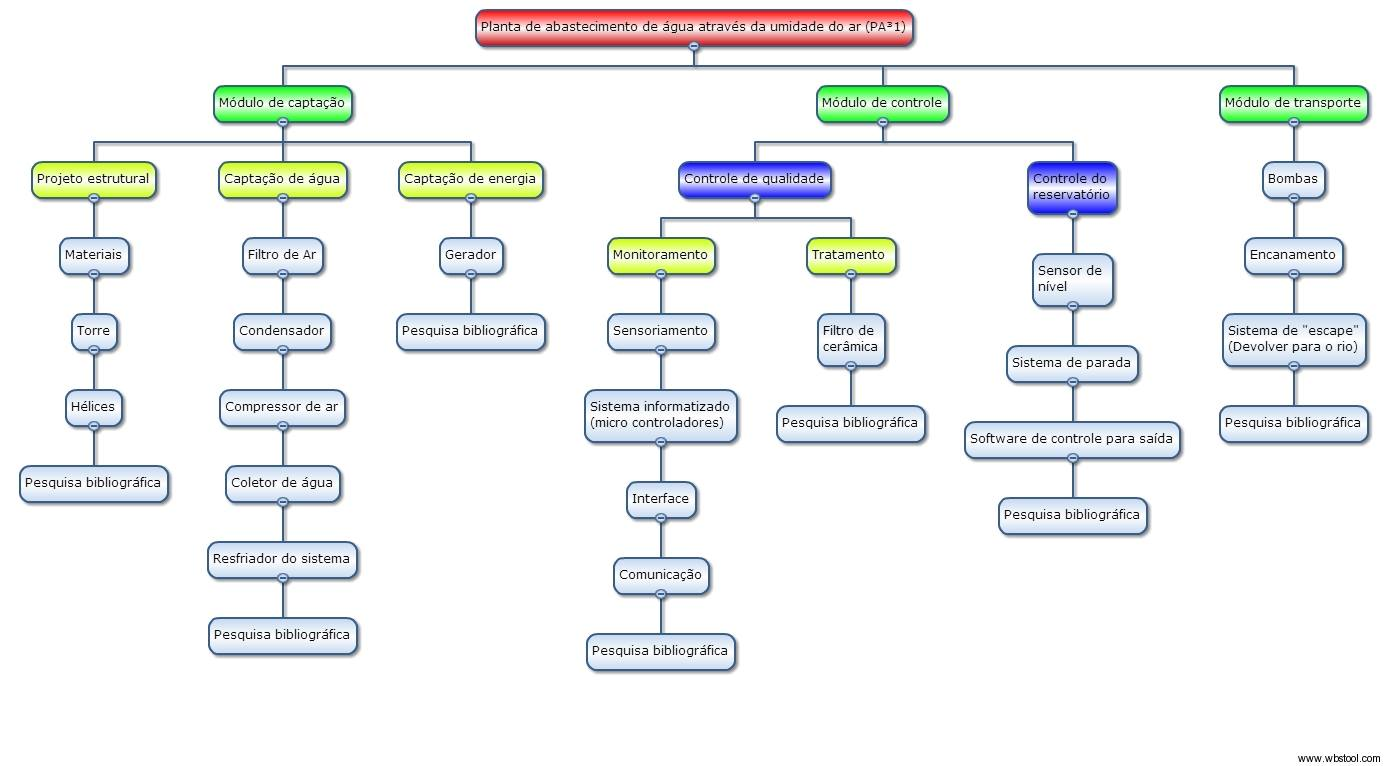
\includegraphics[scale = 0.4, angle=90]{editaveis/figuras/EAP}
    \label{EAP}
    \caption{Estrutura Analítica do Projeto}
   \end{figure}
   \FloatBarrier
   
  \pagebreak
  \subsection{Cronograma}
   
   \textbf{Cronograma de atividades - Ponto de Controle 1}
   \begin{figure}[!h]
    \centering
    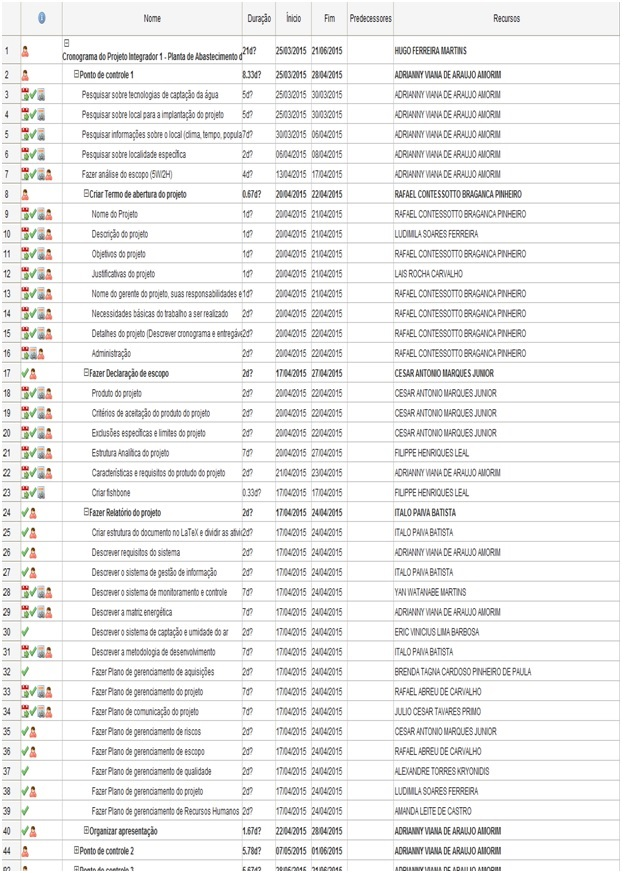
\includegraphics[scale = 0.8]{editaveis/figuras/cronogramaPC1}
    \label{Cronograma de atividades}
    \caption{Cronograma de atividades}
   \end{figure}
   \FloatBarrier
   
   \pagebreak
   \textbf{Cronograma de atividades - Ponto de Controle 2}
   \begin{figure}[!h]
    \centering
    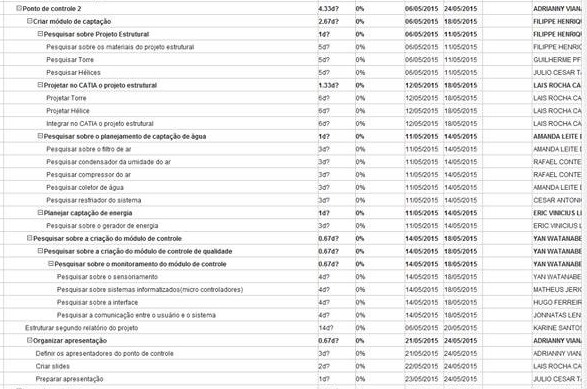
\includegraphics[scale = 0.8]{editaveis/figuras/cronogramaPC2}
    \label{Cronograma de atividades}
    \caption{Cronograma de atividades}
   \end{figure}
   \FloatBarrier
   
   \pagebreak
   \textbf{Cronograma de atividades - Ponto de Controle 3}
   \begin{figure}[!h]
    \centering
     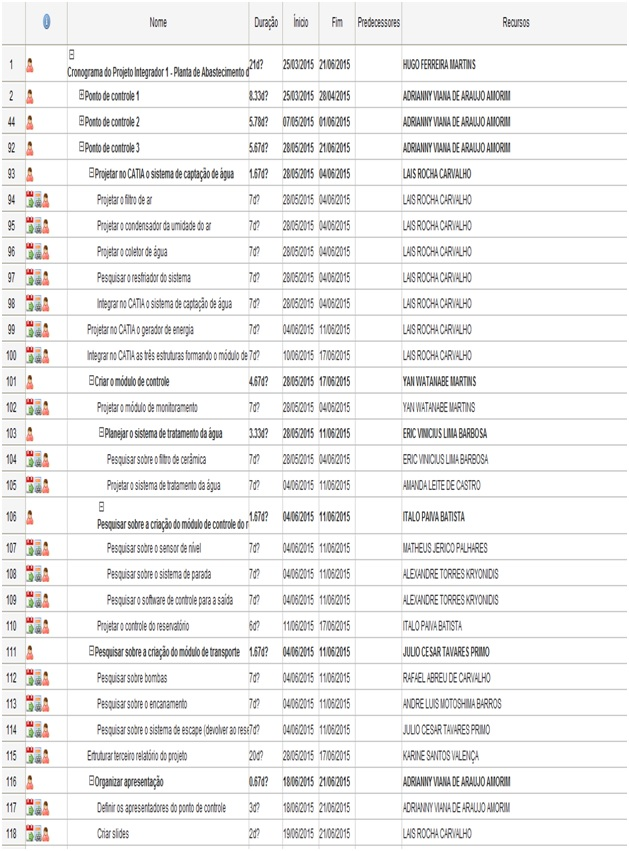
\includegraphics[scale = 0.8]{editaveis/figuras/cronogramaPC3}
    \label{Cronograma de atividades}
    \caption{Cronograma de atividades}
   \end{figure}
   \FloatBarrier
   
  \pagebreak
  \textbf{Gráfico de Gantt- Ponto de Controle 1}
   \begin{figure}[!h]
    \centering
    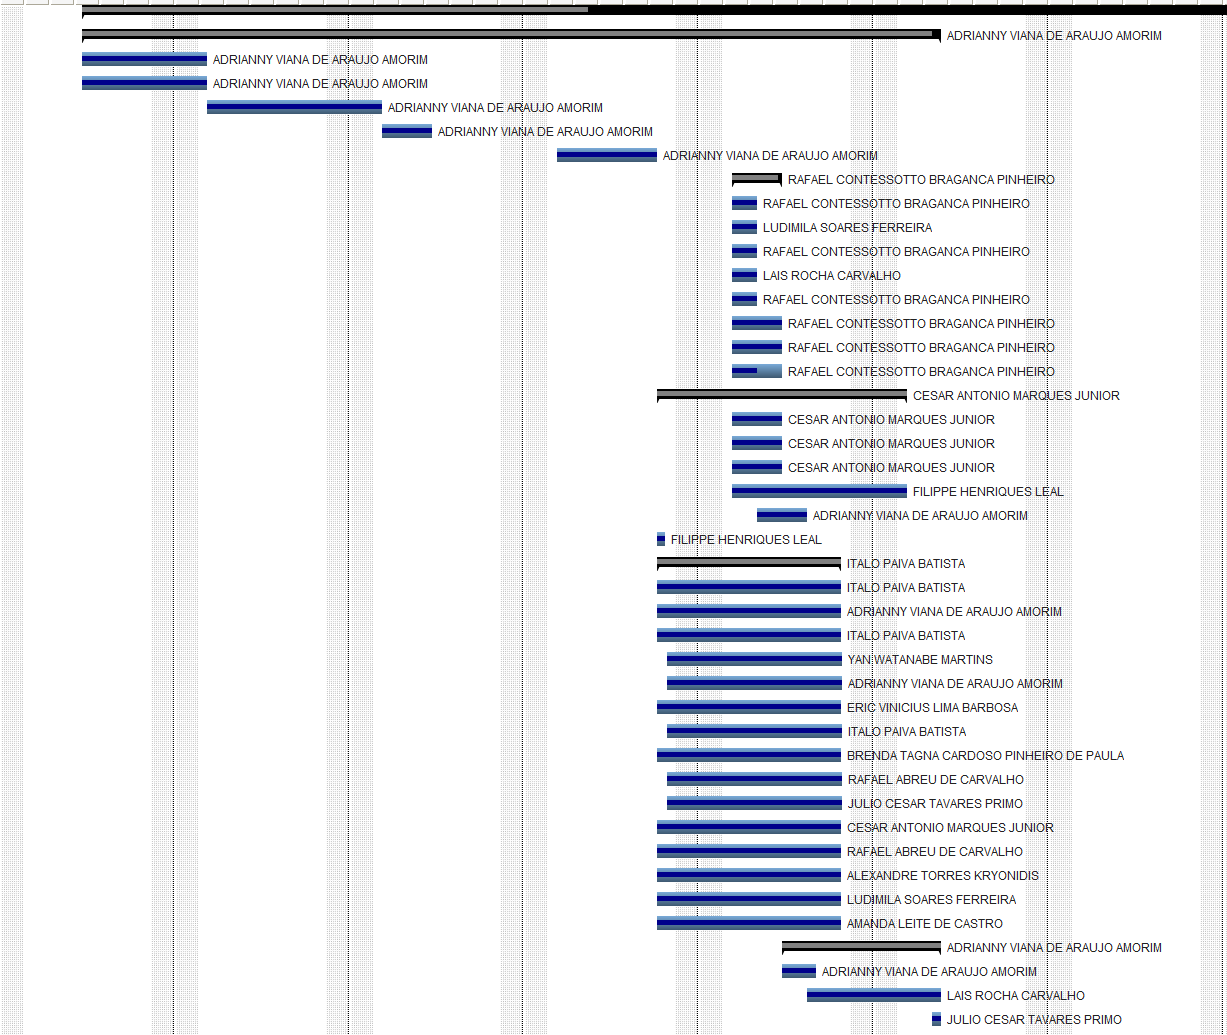
\includegraphics[scale = 0.5]{editaveis/figuras/ganttPC1}
    \label{Gráfico de Gantt}
    \caption{Gráfico de Gantt}
   \end{figure}
   \FloatBarrier
   
  \pagebreak
  \textbf{Gráfico de Gantt- Ponto de Controle 2}
   \begin{figure}[!h]
    \centering
    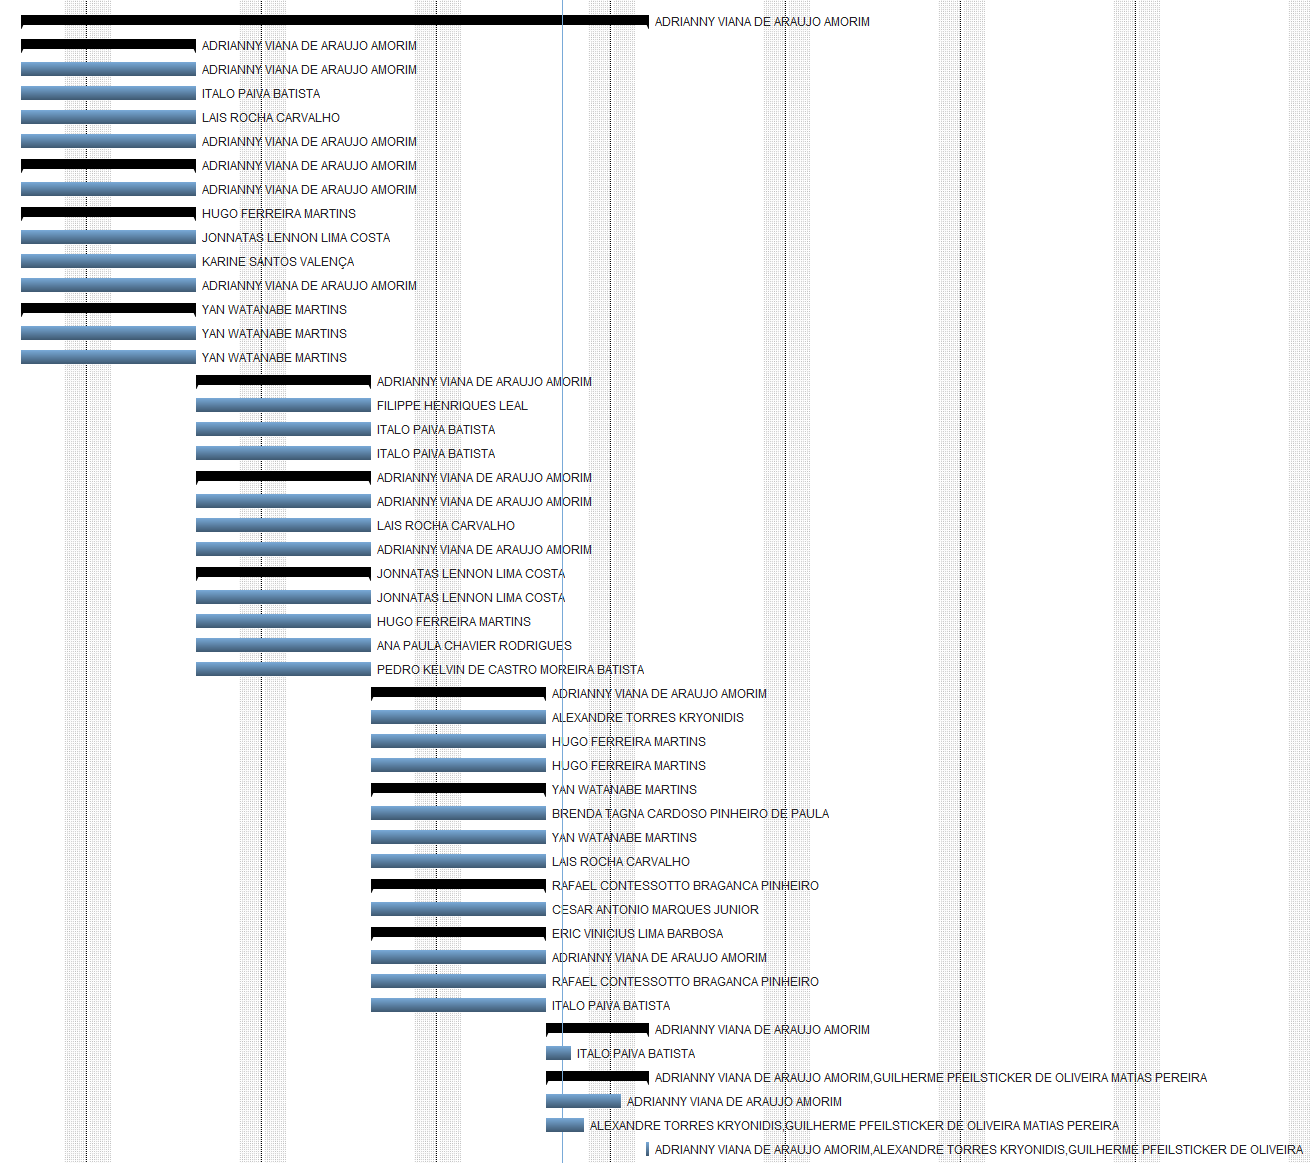
\includegraphics[scale = 0.5]{editaveis/figuras/ganttPC2}
    \label{Gráfico de Gantt}
    \caption{Gráfico de Gantt}
   \end{figure}
   \FloatBarrier
   
  \pagebreak
  \textbf{Gráfico de Gantt- Ponto de Controle 3}
   \begin{figure}[!h]
    \centering
    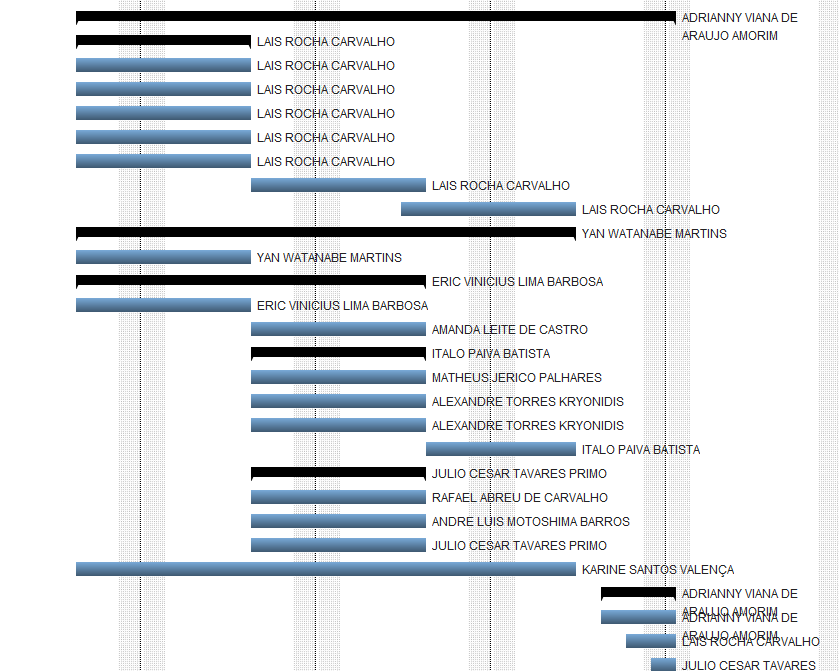
\includegraphics[scale = 0.5]{editaveis/figuras/ganttPC3}
    \label{Gráfico de Gantt}
    \caption{Gráfico de Gantt}
   \end{figure}
   \FloatBarrier